\documentclass[twocolumn,letterpaper,10pt]{article}

\usepackage[margin=0.75in]{geometry}
\usepackage{graphicx}
\usepackage{booktabs}
\usepackage{amsmath, amssymb}
\usepackage{microtype}
\usepackage{xcolor}
\usepackage[round]{natbib}
\usepackage[colorlinks=true,linkcolor=black,citecolor=black,urlcolor=blue!60!black]{hyperref}
\usepackage{caption}
\usepackage{subcaption}
\usepackage{float}
\usepackage{titling}
\usepackage{array}

\setlength{\columnsep}{0.32in}
\setlength{\droptitle}{-0.8in}

\captionsetup{font=small,labelfont=bf,skip=4pt}

\title{\vspace{-0.2in}\textbf{What Makes Good Pretraining Data?\\An Interpretable, Causally-Grounded Answer}}
\author{Kaitlyn Wang, Angikar Ghosal\\Stanford University \textendash{} STATS 305C, Milestone 4}

\begin{document}
\maketitle
\vspace{-0.25in}

%% ============================================================
\section{Changes for this Milestone}
\label{sec:intro}

We revisit our original aim, which is to leverage existing empirical results on data filters to understand what makes a document qualify as "good training data" for language models when compute is limited. In Milestone~3, we 
fit a hierarchical Bayesian model to predict
the \emph{average of existing filter scores} from text features. The
fit was high ($R^2 > 0.7$), but the target was circular, and we lacked an independent ground truth
against which a posterior predictive check could detect failure.

In Milestone~4, we establish ground truth by training small model swarms. We make four substantive revisions.

\textbf{1. Interpretable features only.} We dont allow our model access to blackbox filters such as DCLM, FineWeb-Edu,
and the perplexity-correlations scores. In their place we add $\sim 30$ human-readable features,
inspired by a review of the synthetic-data literature: we measure entity count and entity diversity (following Synthetic Continued Pretraining
\citep{yang2024entigraph} which emphasizes relationships between entities), textbook-like qualities
(following Textbooks~Are~All~You~Need \citep{gunasekar2023textbooks}, which trained Phi models exclusively on data reformatted to textbook-like structure),
and other readability features. 
These features are not only very interpretable, but allow us to confirm/understand what synthetic data people have hypothesized is important for creating more good training data. 

\textbf{2. Ground truth.} A major challenge is, it's quite difficult to obtain a "ground truth" quality score per document. We estimate this by pretraining from scratch a swarm of $593$ small models (15M parameters on 150M tokens, $\sim$20-min train run on GPU) on different
document subsets, which compete on validation loss.
This way, we estimate per-document contributions via
difference-in-means, or \textit{how much does including each document lower
the validation loss of a small LM trained on the mix?}

\textbf{3. Interpretable Model.} Given these input features as well as ground truth quality labels, we now choose to model individual document quality with an Explainable Boosting
Machine (EBM) \citep{lou2013ebm,nori2019interpretml}, which is a
generalised additive model. We like this model because it gives us learned 1-D shape functions of how each feature affects the score, plus
pairwise interactions between features. To confirm that this non-linearity is needed, we also fit Lasso regression as a baseline.

\textbf{4. Validation of Model.} To validate our model, we hold out $30$ shards
($540$M fresh tokens) that were never seen during target construction.
We compare our EBM model selection strategy with baselines such as (DCLM, FineWeb-Edu, Lasso,
random, EBM-within-topic), which are used to select top $150$M quality tokens from the validation pool, and train a larger model
($60$M for $2$ epochs), and evaluate on validation loss plus
downstream benchmarks. This allows us to confirm our model of "quality" beats out existing baselines.

%% ============================================================
\section{Obtaining Ground Truth Document Quality Targets}
\label{sec:target}

We use a randomized experiment difference-in-means
estimator, laid out by previous literature \citep{imbens2015causal,ilyas2022datamodels,engstrom2024dsdm}.
For each document $i$ in the $D=2.06$M-doc training pool, let
$\mathcal{R}_i^+$ and $\mathcal{R}_i^-$ be the runs that include or
exclude it, and let $\ell_r$ be the held-out val loss of run $r$. We
define
\begin{equation}
  y_i \;=\; \frac{1}{|\mathcal{R}_i^-|}\!\sum_{r\in\mathcal{R}_i^-}\!\ell_r
        \;-\; \frac{1}{|\mathcal{R}_i^+|}\!\sum_{r\in\mathcal{R}_i^+}\!\ell_r,
  \label{eq:y}
\end{equation}
so positive $y_i$ means including $i$ tended to lower val loss. We use a variety of subsets to construct this dataset with 593 training runs total. Each
document appears in $\sim 50.6$ runs on average. The split-half Pearson
reliability of $y$ is $0.40$, which implies a noise-limited $R^2$ ceiling
of $\approx 0.57$--$0.70$ for any feature-based predictor of $y$.

\paragraph{Subset construction.} Causal identification requires that
the inclusion pattern of $i$ across runs is not collinear with that
of every other document. However in practice, we also want a broad coverage of
real-world selection strategies. We designed $791$ subsets across
five families (Table~\ref{tab:strategies}); after enforcing a minimum of
$150$M unique tokens for each strategy, we are left with $593$ subsets total.

\begin{table}[t]
\small
\centering
\begin{tabular}{p{1.6cm} p{4.2cm} r}
\toprule
Strategy & Example & Runs \\
\midrule
Random threshold & top-$15\%$ by \texttt{entity\_density} & 200 \\
Multi-feature intersection & top-$30\%$ entity AND top-$30\%$ \texttt{discourse\_causal} & 300 \\
Linear combination & top-$15\%$ by random $w^{\!\top} x$, $w\sim\mathcal{N}(0,I)$ & 200 \\
Targeted / baseline & top-$15\%$ by DCLM, FineWeb-Edu, QuRater axes, random samples & 50 \\
Topic-conditional & top-$30\%$ by \texttt{textbook\_quality}, within Health topic & 50 \\
\bottomrule
\end{tabular}
\caption{5 strategies we used to construct the subsets that
feed $y$. A total of $593$ of $791$ designed
runs were trained.}
\label{tab:strategies}
\end{table}

%% ============================================================
\section{Interpretable Models of Quality}
\label{sec:models}

With $y$ in hand, we fit two predictors from the $44$+$2$ feature
panel. \textbf{Lasso} is an $L_1$-regularised linear regression with
cross-validated penalty; it provides a faithful linear baseline.
\textbf{EBM} is a generalized additive model
$\hat{y}(x)=\sum_k f_k(x_k)+\sum_{j<k} f_{jk}(x_j,x_k)$ whose 1-D
shape functions $f_k$ and pairwise interactions $f_{jk}$ are directly
visualizable. We pick the EBM because (i)~we suspected non-linear
effects (sweet spots, saturation), which the $R^2$ comparison
(Table~\ref{tab:r2}) confirms, and (ii)~it lets us read off, per
feature, exactly how the model believes that feature affects quality.


On a $20\%$ stratified held-out split ($412$K docs), the EBM reaches
$R^2 = 0.67$. Lasso achieves only $0.41$, confirming that
non-linearity and feature interactions are doing substantial work.
Noticeably, we found training $R^2$ is also $0.67$, indicating the EBM has hit the
intrinsic noise ceiling of $y$ rather than overfitting. Unfortunately our estimates from training real model checkpoints are quite noisy; a more principled approach might be to use metagradients to do data attribution, which is a lot more complicated to set up, but we consider exploring in next steps.

\paragraph{EBM model interpretation \& results.}
Figure~\ref{fig:imp} gives the top-$12$ most important features and
whether each has a monotone-positive ($\uparrow$), monotone-negative
($\downarrow$), or peaked-sweet-spot ($\cap$) effect on $y$.
Educational tone, textbook style, and proper-noun usage dominate. The
full learned shape functions for the top six features are in
Figure~\ref{fig:appx_shapes} (appendix). Educational tone is
monotone-positive and the single strongest signal; textbook quality is
important but saturates above $\sim 0.5$; proper-noun density and
first-person voice both have \emph{steep penalty regions} away from
their sweet spots (e.g.\ too-high entity density flags entity-dump
list pages). We also manually reviewed documents at the 10th, 50th,
and 90th percentiles of the most important features to confirm these
patterns by eye.

\begin{figure}[t]
  \centering
  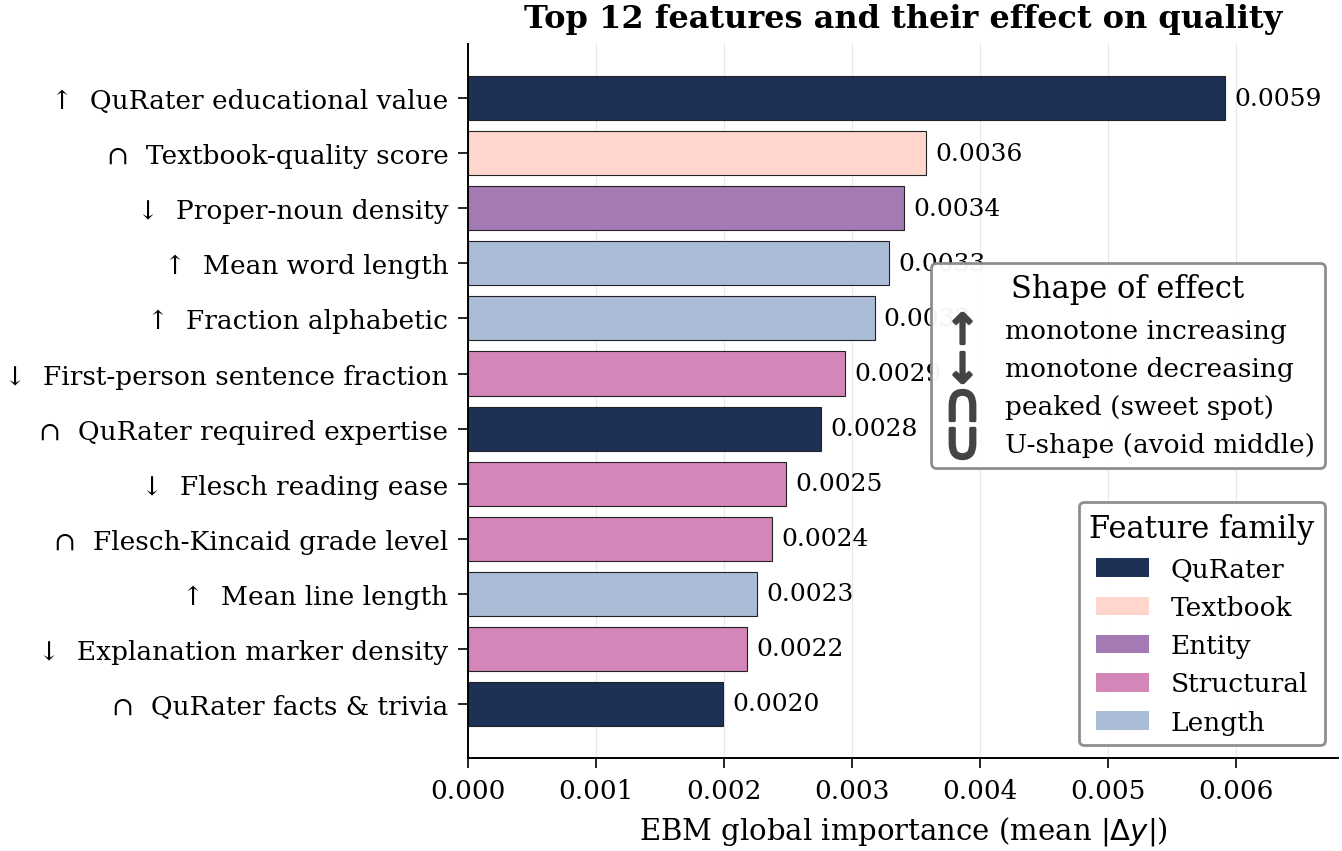
\includegraphics[width=\columnwidth]{fig_ebm_importance.png}
  \caption{Top-$12$ EBM features ranked by global importance. Glyphs:
  $\uparrow$ monotone increasing, $\downarrow$ monotone decreasing,
  $\cap$ peaked sweet-spot.}
  \label{fig:imp}
\end{figure}

%% ============================================================
\section{Downstream Validation}
\label{sec:validation}

An interpretable model is only useful if its predictions translate to
performant LMs. We validate the EBM as a \emph{selection policy}
on $30$ freshly downloaded shards ($612$K docs, $540$M tokens)
disjoint from every earlier phase. For each strategy we picked
exactly $150$M unique tokens by that strategy's criterion, trained a
$60$M Llama for $2$ epochs ($300$M total training tokens), and
evaluated on four metrics: held-out CommonCrawl perplexity (CC val),
HellaSwag accuracy \citep{zellers2019hellaswag}, ARC-Easy accuracy
\citep{clark2018arc}, and LAMBADA loss \citep{paperno2016lambada}.

%% ============================================================
\section{Results}
\label{sec:results}

The results are mixed: \emph{no single strategy wins on every metric},
and the strategies that win on broad CC perplexity lose on factual
benchmarks. The full per-metric comparison is in
Table~\ref{tab:bench}.

\textbf{Within-topic EBM matches the best random run.} EBM-within-topic
(an OLMo-3 style protocol \citep{olmo3} that selects the top
EBM-scored docs \emph{within each topic}) is best on CC validation
($3.873$ vs.\ random's $3.884$) and HellaSwag ($31.95\%$ vs.\
$31.50\%$). This is the only filter strategy that does not lose to
random on broad CC perplexity.

\textbf{Every global top-$k$ filter loses to random on CC.}
DCLM, FineWeb-Edu, EBM, and Lasso all underperform random by
$0.02$--$0.13$ nats on broad CommonCrawl validation. This was quite interesting to us; we think the most
plausible explanation is distribution narrowing
\citep{naitsaada2025illusion}: training on a stylistically narrow ``high quality''
slice hurts a model's performance on predicting low quality data on the val set.

\textbf{Filter purpose matters more than ``quality.''} We do also confirm that DCLM,
trained specifically to lift downstream benchmark performance, does not win on broad perplexity but wins on specific downstream tasks. Our EBM is the inverse
trade-off - it wins on broad predict next token objectives and loses on factual recall/downstream tasks. This concretely reproduces the ``Data Quality Illusion''
\citep{naitsaada2025illusion}: there is no single ``quality'' axis;
each filter optimizes against its training reference and predictably
loses elsewhere.

%% ============================================================
\section{Limitations}
\label{sec:limitations}

\textbf{Noise ceiling on $y$.} The EBM achieves $R^2 = 0.66$ on the
training data as well as the validation data. This indicates we have
hit the intrinsic noise ceiling of $y$, not a modelling failure. We have already invested quite a bit of compute with $593$ small-model runs and ~$50$ inclusions per document, but more diagnostic runs would help lift this ceiling. Metagradients could also provide a more principled approach to data attribution.

\textbf{Choice of validation set.} Every choice biases some direction.
A curated set like Wikipedia would inflate FineWeb-Edu / educational
filters by construction. Held-out raw CC favors random selection
because the corpus itself is heavy on low-quality material, and DCLM
explicitly trades short-term CC perplexity for downstream benchmark
gains. We therefore report both: broad CC validation \emph{and} three
downstream tasks (HellaSwag, ARC-Easy, LAMBADA), so that no single
choice of metric determines the conclusion.

\textbf{Scale.} Validation uses $60$M models trained on $300$M
tokens. At the $1$B-parameter / $25$B-token scale where DCLM was
originally evaluated, the relative ordering may shift; our finding
that ``no single filter wins'' may itself be scale-dependent.

\textbf{Selection-strategy bias in $y$.} The diagnostic mix
distribution is biased toward random and single-feature subsets;
\citet{engstrom2024dsdm} note that including selection-style mixes in
the diagnostic set is important for top-$k$ generalisation, which we
do only partially.

\textbf{Synthetic data} An interesting next step we are thinking about is to apply this feature pipeline to
\emph{synthetic} pretraining data --- Cosmopedia, OpenHermes-2.5,
WildChat --- and ask whether our learned shape functions distinguish
synthetic from real-world text. 
%% ============================================================

\small
\bibliographystyle{plainnat}
\begin{thebibliography}{99}

\bibitem[Clark et al.(2018)]{clark2018arc}
P.~Clark, I.~Cowhey, O.~Etzioni, T.~Khot, A.~Sabharwal, C.~Schoenick,
O.~Tafjord.
\newblock Think You Have Solved Question Answering? Try ARC, the AI2
  Reasoning Challenge.
\newblock \emph{arXiv:1803.05457}, 2018.

\bibitem[Engstrom et al.(2024)]{engstrom2024dsdm}
L.~Engstrom, A.~Feldmann, A.~Madry.
\newblock DsDm: Model-Aware Dataset Selection with Datamodels.
\newblock \emph{ICML}, 2024.

\bibitem[Gunasekar et al.(2023)]{gunasekar2023textbooks}
S.~Gunasekar et al.
\newblock Textbooks Are All You Need.
\newblock \emph{arXiv:2306.11644}, 2023.

\bibitem[Ilyas et al.(2022)]{ilyas2022datamodels}
A.~Ilyas, S.~M.~Park, L.~Engstrom, G.~Leclerc, A.~Madry.
\newblock Datamodels: Predicting Predictions from Training Data.
\newblock \emph{NeurIPS}, 2022.

\bibitem[Imbens \& Rubin(2015)]{imbens2015causal}
G.~W.~Imbens, D.~B.~Rubin.
\newblock \emph{Causal Inference for Statistics, Social, and Biomedical
  Sciences}.
\newblock Cambridge University Press, 2015.

\bibitem[Li et al.(2024)]{li2024dclm}
J.~Li et al.
\newblock DataComp-LM: In Search of the Next Generation of Training
  Sets for Language Models.
\newblock \emph{arXiv:2406.11794}, 2024.

\bibitem[Lou et al.(2013)]{lou2013ebm}
Y.~Lou, R.~Caruana, J.~Gehrke, G.~Hooker.
\newblock Accurate Intelligible Models with Pairwise Interactions.
\newblock \emph{KDD}, 2013.

\bibitem[Nait Saada et al.(2025)]{naitsaada2025illusion}
Y.~Nait~Saada et al.
\newblock The Data Quality Illusion: Rethinking Classifier-Based
  Quality Filtering for LLM Pretraining.
\newblock \emph{arXiv preprint}, 2025.

\bibitem[Nori et al.(2019)]{nori2019interpretml}
H.~Nori, S.~Jenkins, P.~Koch, R.~Caruana.
\newblock InterpretML: A Unified Framework for Machine Learning
  Interpretability.
\newblock \emph{arXiv:1909.09223}, 2019.

\bibitem[OLMo Team(2025)]{olmo3}
OLMo Team.
\newblock OLMo~3: Open Language Models with Open Training Data.
\newblock \emph{Tech report}, 2025.

\bibitem[Paperno et al.(2016)]{paperno2016lambada}
D.~Paperno et al.
\newblock The LAMBADA Dataset: Word Prediction Requiring a Broad
  Discourse Context.
\newblock \emph{ACL}, 2016.

\bibitem[Penedo et al.(2024)]{penedo2024fineweb}
G.~Penedo et al.
\newblock The FineWeb Datasets: Decanting the Web for the Finest Text
  Data at Scale.
\newblock \emph{NeurIPS}, 2024.

\bibitem[Thrush et al.(2025)]{thrush2024perplexity}
T.~Thrush, C.~Potts, T.~Hashimoto.
\newblock Improving Pretraining Data Using Perplexity Correlations.
\newblock \emph{ICLR}, 2025.

\bibitem[Wettig et al.(2024)]{wettig2024qurating}
A.~Wettig, T.~Gao, S.~Zhao, D.~Chen.
\newblock QuRating: Selecting High-Quality Data for Training Language
  Models.
\newblock \emph{ICML}, 2024.

\bibitem[Wettig et al.(2025)]{wettig2025weborganizer}
A.~Wettig, K.~Lo, S.~Min, H.~Hajishirzi, D.~Chen, P.~Dasigi.
\newblock Organize the Web: Constructing Domains Enhances Pre-Training
  Data Curation.
\newblock \emph{ICML}, 2025.

\bibitem[Yang et al.(2024)]{yang2024entigraph}
Z.~Yang, N.~Band, S.~Li, E.~Cand\`es, T.~Hashimoto.
\newblock Synthetic Continued Pretraining.
\newblock \emph{ICLR}, 2025.

\bibitem[Zellers et al.(2019)]{zellers2019hellaswag}
R.~Zellers, A.~Holtzman, Y.~Bisk, A.~Farhadi, Y.~Choi.
\newblock HellaSwag: Can a Machine Really Finish Your Sentence?
\newblock \emph{ACL}, 2019.
\end{thebibliography}

%% ============================================================
\onecolumn
\appendix
\section*{Appendix: Additional Tables and Figures}

\begin{table}[h]
\small
\centering
% Auto-generated. Bold = best on this metric; underlined = worst on this metric.
\begin{tabular}{lcccc}
\toprule
Selection strategy & CC val loss & HellaSwag & ARC-Easy & LAMBADA loss \\
 & (nats $\downarrow$) & (acc $\uparrow$) & (acc $\uparrow$) & (nats $\downarrow$) \\
\midrule
Random (seed 42) & 3.884 & 0.313 & 0.349 & 4.528 \\
Random (seed 43) & 3.887 & 0.315 & 0.332 & 4.564 \\
Random (seed 44) & 3.896 & 0.311 & 0.340 & 4.501 \\
EBM within-topic & \textbf{3.873} & \textbf{0.320} & \underline{0.316} & 4.724 \\
EBM-full & 3.914 & 0.308 & 0.337 & 5.168 \\
EBM-no-PC & 3.921 & 0.307 & 0.326 & 5.169 \\
EBM-full (seed 43) & 3.918 & 0.311 & 0.326 & 5.212 \\
Lasso & 3.960 & \underline{0.303} & 0.370 & \underline{5.307} \\
DCLM-fastText & \underline{4.006} & 0.304 & \textbf{0.379} & \textbf{4.350} \\
FineWeb-Edu & 3.967 & 0.308 & 0.365 & 4.746 \\
\bottomrule
\end{tabular}

\caption{Performance of each data selection strategy on held out validation set. $60$M Llama models trained
on $150$M unique tokens per strategy. Each downstream metric produces its own ranking of strategies. \textbf{Bold} = best,
\underline{underlined} = worst per column.}
\label{tab:bench}
\end{table}

% ---- Three figures (shapes, calibration, R^2 bar) packed onto a single page ----
\clearpage

\begin{figure}[H]
  \centering
  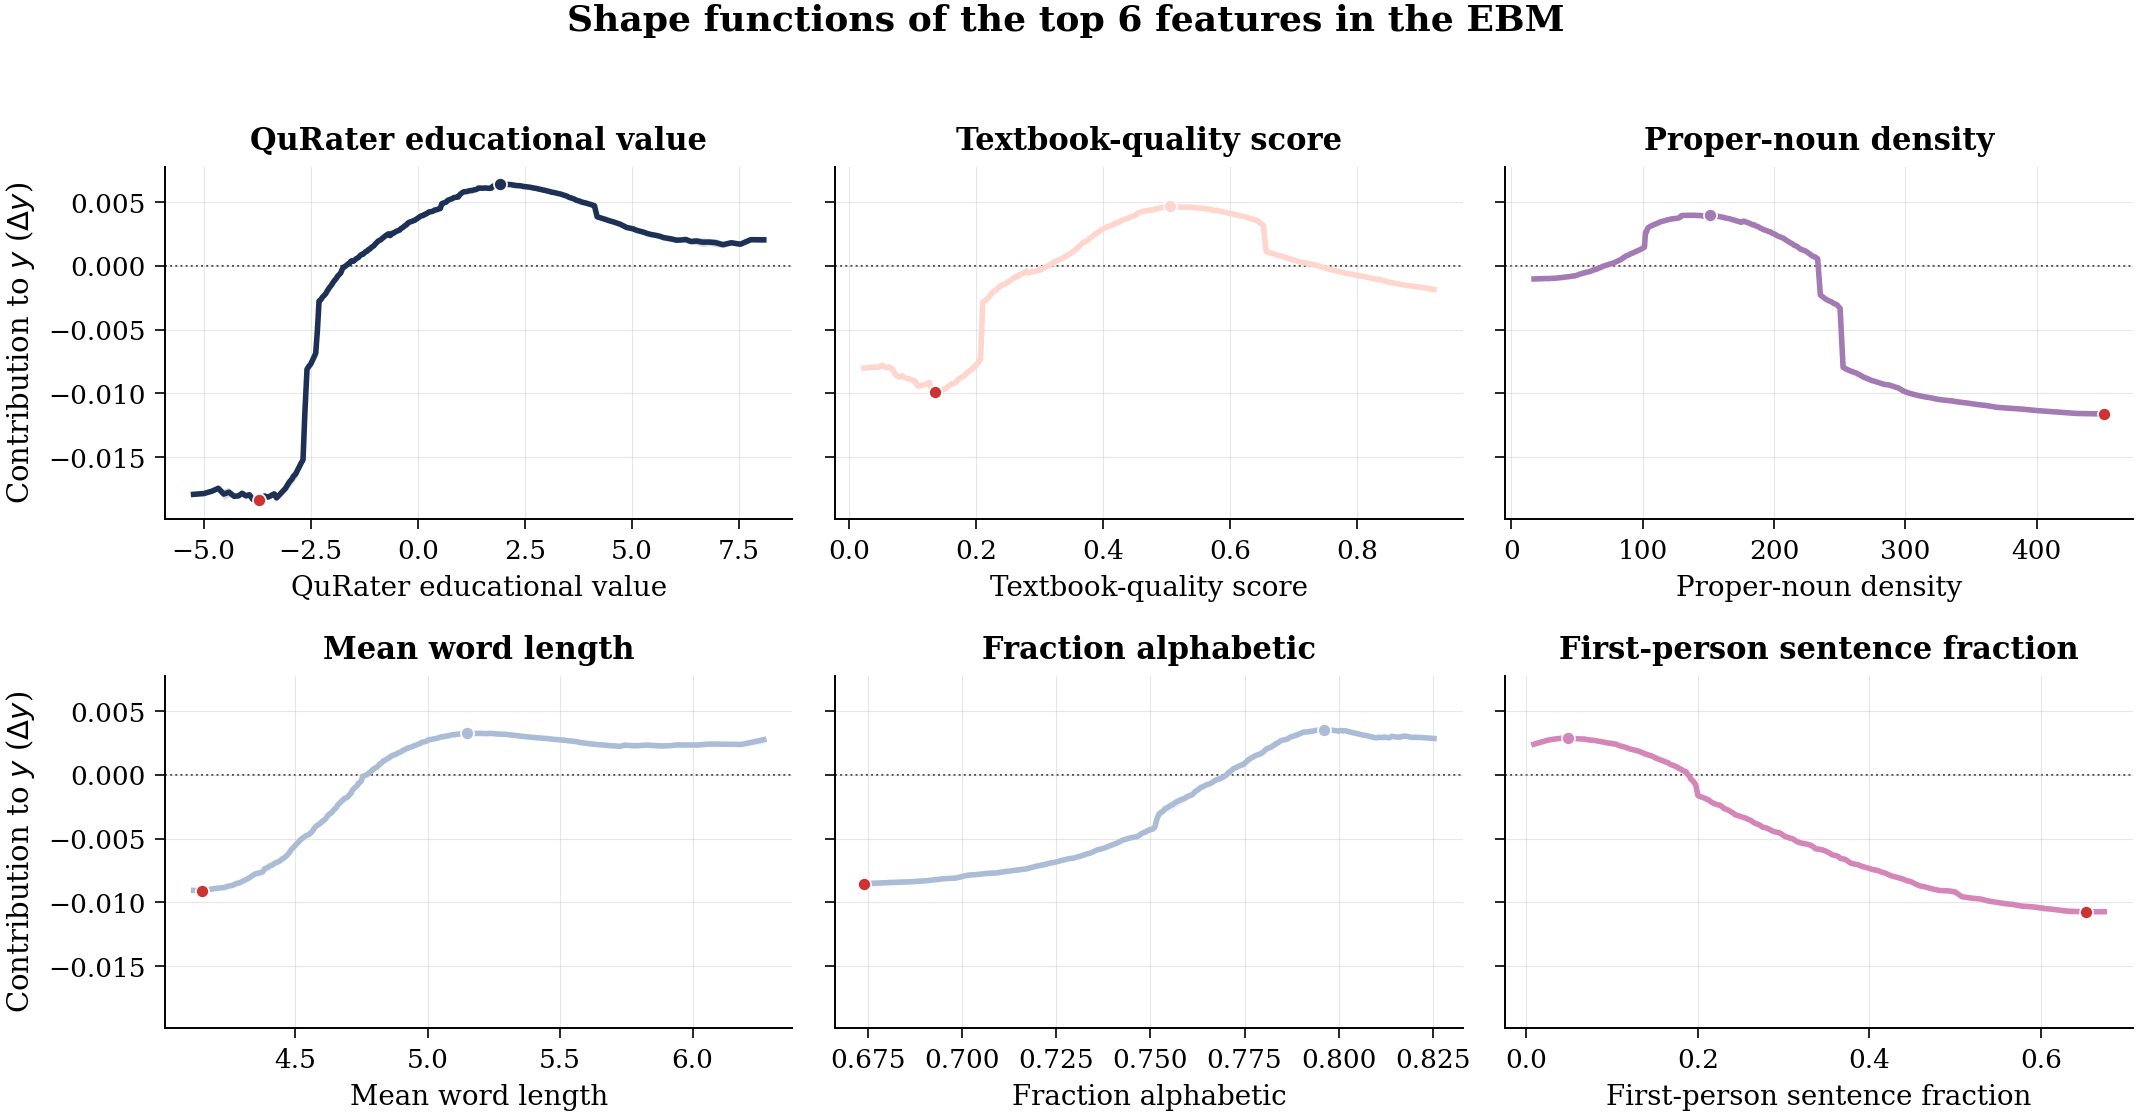
\includegraphics[width=0.92\textwidth]{fig_ebm_shapes.png}
  \caption{EBM 1-D shape functions for the top six features with
  $95\%$ bag-bootstrap bands. Colored dots mark the model's argmax
  (sweet spot); red dots mark the argmin (penalty region).}
  \label{fig:appx_shapes}
\end{figure}

\vspace{6pt}

\noindent\begin{minipage}[t]{0.48\textwidth}
  \centering
  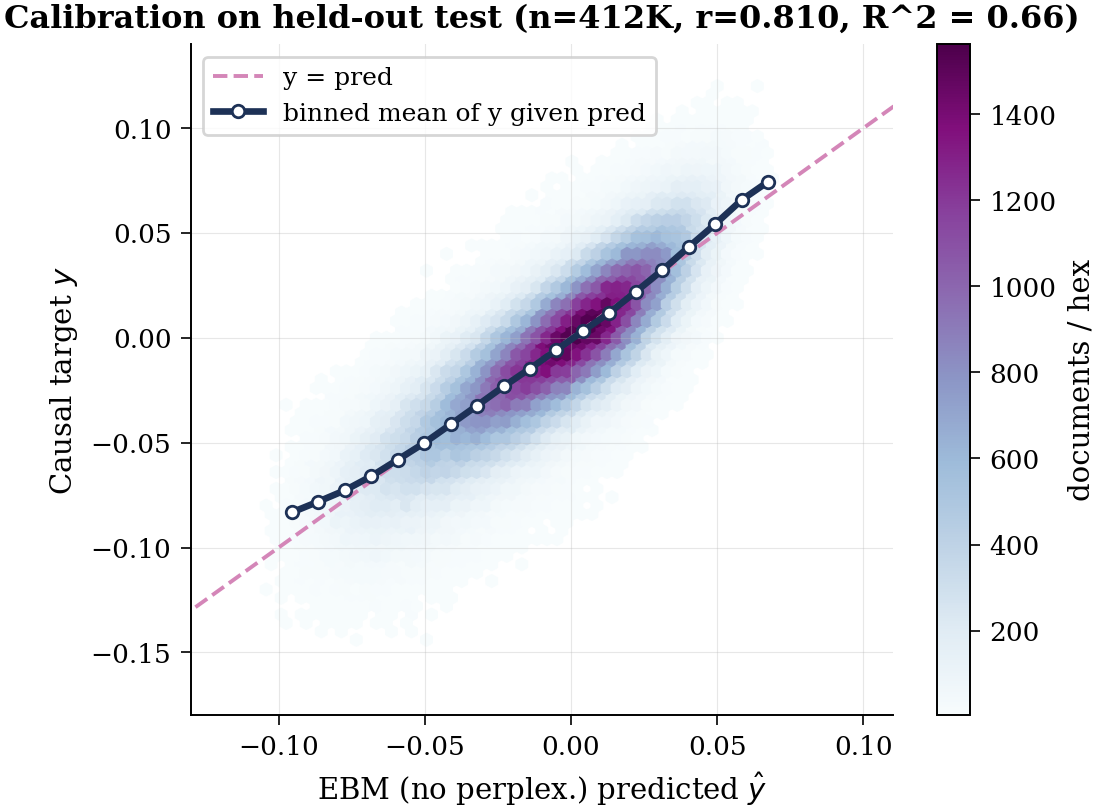
\includegraphics[width=0.95\textwidth]{fig_calibration.png}
  \captionof{figure}{Calibration of the EBM on the
  held-out $412$K-doc test set. The binned mean of $y$ given
  $\hat{y}$ (navy curve) tracks the diagonal closely across the
  prediction range.}
  \label{fig:appx_cal}
\end{minipage}\hfill
\begin{minipage}[t]{0.48\textwidth}
  \centering
  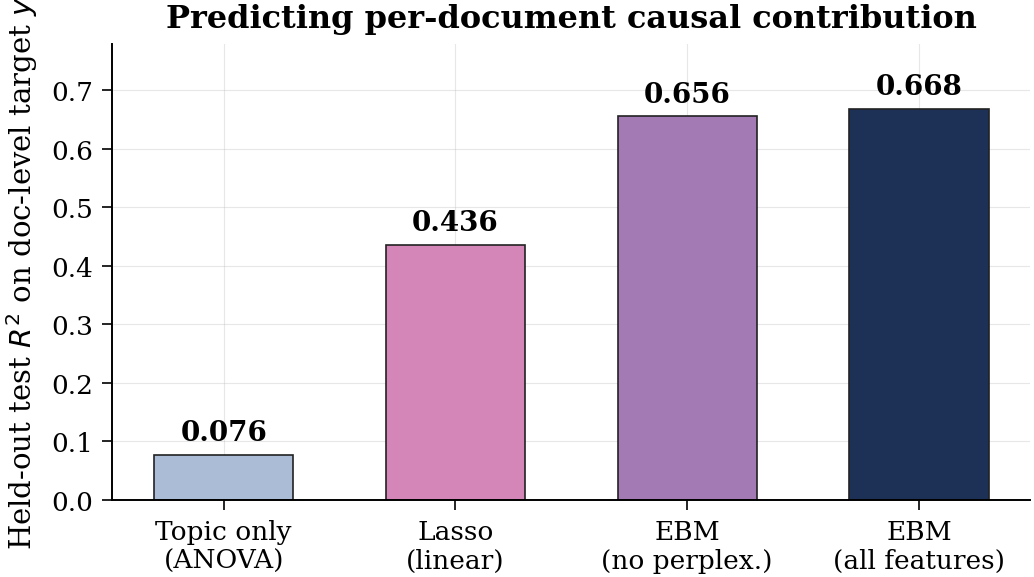
\includegraphics[width=0.95\textwidth]{fig_model_r2.png}
  \captionof{figure}{Held-out test $R^2$ for the three predictors of
  $y$ as a bar chart (numeric form in Table~\ref{tab:r2}).}
  \label{fig:appx_r2bar}
\end{minipage}

\end{document}
